\documentclass[10pt,letterpaper,notitlepage]{article}
\usepackage[utf8]{inputenc}
\usepackage{amsmath}
\usepackage{amsfonts}
\usepackage{amssymb}
\usepackage{graphicx}
\usepackage{cancel}
\usepackage{float}
\usepackage{cite}

\usepackage[ruled,vlined]{algorithm2e}


\usepackage[left=0.75in, right=0.75in, bottom=1.0in,top=0.75in]{geometry}

%\usepackage{caption} 
%\captionsetup[table]{skip=10pt}
%\usepackage[font=small,labelfont=bf]{caption}

\usepackage{comment}
\usepackage{listings}

\usepackage{color}
\definecolor{Brown}{cmyk}{0,0.81,1,0.60}
\definecolor{OliveGreen}{cmyk}{0.64,0,0.95,0.40}
\definecolor{CadetBlue}{cmyk}{0.62,0.57,0.23,0}

\usepackage{multicol}

\usepackage{appendix}

\usepackage{fancyhdr}
%\usepackage[colorlinks=true,linkcolor=blue,urlcolor=black,bookmarksopen=true,bookmarks]{hyperref}
\usepackage{bookmark}

\numberwithin{equation}{section} 


%============================= Put document title here
\newcommand{\DOCTITLE}{Compressible inviscid fluid flow solver using the MUSCLE-Hancock method and a HLLC Riemann solver.}  

%=============================  Load list of user-defined commands
% Mark URL's
\newcommand{\URL}[1]{{\textcolor{blue}{#1}}}
%
% Ways of grouping things
%
\newcommand{\bracket}[1]{\left[ #1 \right]}
\newcommand{\bracet}[1]{\left\{ #1 \right\}}
\newcommand{\fn}[1]{\left( #1 \right)}
\newcommand{\ave}[1]{\left\langle #1 \right\rangle}
\newcommand{\norm}[1]{\Arrowvert #1 \Arrowvert}
\newcommand{\abs}[1]{\arrowvert #1 \arrowvert}
%
% Partial derivative
\newcommand{\partialderiv}[2]{\frac{\partial #1}{\partial #2}}
%
% Bold quantities
% 
\newcommand{\Omegabf}{\mathbf{\Omega}}
\newcommand{\bnabla}{\boldsymbol{\nabla}}
\newcommand{\position}{\mathbf{x}}
\newcommand{\velocity}{\mathbf{u}}
\newcommand{\dotp}{\boldsymbol{\cdot}}

\newcommand{\uvec}[1]{\boldsymbol{\hat{\textbf{#1}}}}

\newcommand{\ihat}{\uvec{\i}}
\newcommand{\jhat}{\uvec{\j}}
\newcommand{\khat}{\uvec{k}}

\newcommand{\hatbf}[1]{\hat{\mathbf{#1}}}

%\newcommand{\ihat}{\boldsymbol{\hat{\textbf{\i}}}}
%\newcommand{\jhat}{\boldsymbol{\hat{\textbf{\j}}}}
%\newcommand{\khat}{\boldsymbol{\hat{\textbf{\k}}}}

%\newcommand{\ihat}{{\bm{\hat{\textnormal{\bfseries\i}}}}}
%\newcommand{\jhat}{{\bm{\hat{\textnormal{\bfseries\j}}}}}
%\newcommand{\khat}{{\bm{\hat{\textnormal{\bfseries\k}}}}}
%
% Vector forms
%
\renewcommand{\vec}[1]{\mbox{$\stackrel{\longrightarrow}{#1}$}}
\renewcommand{\div}{\mbox{$\vec{\mathbf{\nabla}} \cdot$}}
\newcommand{\grad}{\mbox{$\vec{\mathbf{\nabla}}$}}
\newcommand{\bb}[1]{\bar{\bar{#1}}}
%
% Vector forms boldfaced
\newcommand{\bvec}[1]{\mathbf{#1}}
\newcommand{\bdiv}{\boldsymbol{\nabla} \boldsymbol{\cdot}}
\newcommand{\bgrad}{\bnabla}
\newcommand{\mat}[1]{\bar{\bar{#1}}}
%
%
% Equation beginnings and endings
%
% Un-numbered equation with alignment
\newcommand{\beq}{\begin{equation*} \begin{aligned}}
\newcommand{\eeq}{\end{aligned}\end{equation*}}
% Numbered equation with alignment
\newcommand{\beqn}{\begin{equation}\begin{aligned}}
\newcommand{\eeqn}{\end{aligned}\end{equation}}  

%
% Quick commands for symbols
%
\newcommand{\Edensity}{\mathcal{E}}


\newcommand{\jcr}[1]{\textcolor{magenta}{#1}}
\usepackage[normalem]{ulem}
\newcommand{\ssout}[1]{\sout{\textcolor{magenta}{#1}}}

%
% Code syntax highlighting
%
%\lstset{language=C++,frame=ltrb,framesep=2pt,basicstyle=\linespread{0.8} \small,
%	keywordstyle=\ttfamily\color{OliveGreen},
%	identifierstyle=\ttfamily\color{CadetBlue}\bfseries,
%	commentstyle=\color{Brown},
%	stringstyle=\ttfamily,
%	showstringspaces=true,
%	tabsize=2,}

\lstset{language=C++,frame=ltrb,framesep=8pt,basicstyle=\linespread{0.8} \Large,
commentstyle=\ttfamily\color{OliveGreen},
keywordstyle=\ttfamily\color{blue},
identifierstyle=\ttfamily\color{CadetBlue}\bfseries,
stringstyle=\ttfamily,
tabsize=2,
showstringspaces=false,
numbers=left,
captionpos=t}

\renewcommand{\lstlistingname}{\textbf{Code Snippet}}% Listing -> Code Snippet


\begin{document}
\noindent
{\LARGE\textbf{\DOCTITLE}}
\newline
\newline
\newline
\noindent
{\Large Jan I.C. Vermaak$^{1,2}$, Jim E. Morel$^{1,2}$}
\newline
\noindent\rule{\textwidth}{1pt}
{\small $^1$Center for Large Scale Scientific Simulations, Texas A\&M Engineering Experiment Station, College Station, Texas, USA.}
\newline\noindent
{\small $^2$Nuclear Engineering Department, Texas A\&M University, College Station, Texas, USA.}
\newline
\newline
\textbf{Abstract:}\newline\noindent
Work is work for some, but for some it is play.
\newline
\newline\noindent
{\small
\textbf{Keywords:} hydrodynamics}

\section{Introduction}
For this research we develop a fluid flow solver for the solution of flow problems involving compressible inviscid ideal gases. The governing equations are the Euler equations defined as
\beqn 
\partialderiv{\rho}{t} + \bnabla \dotp (\rho \velocity) = 0
\eeqn 
\beqn 
\partialderiv{(\rho\velocity)}{t} + \bnabla \dotp \{ \rho \velocity \otimes \velocity\}  + \bnabla P = \mathbf{f}
\eeqn 
\beqn 
\partialderiv{E}{t} + \bnabla \dotp [(E + p)\velocity] = q,
\eeqn 
where $\rho$ is the fluid density, $\velocity = [u_x, u_y, u_z] =[u,v,w]$ is the fluid velocity in cartesian coordinates, $P$ is the fluid pressure, $\mathbf{f} = [f_x,f_y,f_z]$ is an arbitrary momentum-density source or sink, $E$ is the material energy-density comprising kinetic energy-density, $\frac{1}{2} \rho ||\velocity||^2$, and internal energy-density, $\rho e$, such that $E = \frac{1}{2} \rho ||\velocity||^2 + \rho e$, where $e$ is the specific internal energy. The value $q$ is an arbitrary energy-density source or sink.

The ideal gas law provides the closure relation
\beqn 
p = (\gamma - 1) \rho e
\eeqn 
where $\gamma$ is the ratio of the constant-pressure specific heat, $c_p$, to the constant-volume specific heat, $c_v$, i.e., $\gamma = \frac{c_p}{c_v}$, and is a material property.

\vspace{1cm}
\subsection{Notation in preparation for numerical schemes}
The conservation of mass-, momentum-, and energy equations can be written in the following form
\beqn \label{eq:euler_operator_form}
\partialderiv{\mathbf{U}}{t} + 
\partialderiv{}{x}\mathbf{F}(\mathbf{U}) +
\partialderiv{}{y}\mathbf{G}(\mathbf{U}) +
\partialderiv{}{z}\mathbf{H}(\mathbf{U}) 
&= 
 \mathbf{Q} \\
\eeqn 
where
\beqn 
\mathbf{U} = 
\begin{bmatrix}
\rho \\ 
\rho u \\
\rho v \\
\rho w \\ 
E
\end{bmatrix}
, \quad 
\mathbf{F}(\mathbf{U})=
\begin{bmatrix}
\rho u \\
\rho uu + p\\
\rho uv \\
\rho uw \\
u(E+p)
\end{bmatrix}
,
\mathbf{G}(\mathbf{U})=
\begin{bmatrix}
\rho v \\
\rho v u \\
\rho vv + p \\
\rho vw \\
v(E+p)
\end{bmatrix}
,
\mathbf{H}(\mathbf{U})=
\begin{bmatrix}
\rho w \\
\rho wu \\
\rho wv \\
\rho ww + p \\
w(E+p)
\end{bmatrix}
, \text{ and }
\mathbf{Q} = 
\begin{bmatrix}
0 \\
f_x \\
f_y \\
f_z \\
q
\end{bmatrix}.
\eeqn 
The $\mathbf{U}$ vector is now a collection of the conserved variables, 
the $\mathbf{F}$, $\mathbf{G}$ and $\mathbf{H}$ vectors is representative of generic flux terms, and the $\mathbf{Q}$ vector is a generic source term. We will be using this notation in the sections that follow.
4


\vspace{1cm}
\subsection{General Finite Volume discretization}
Consider the cell volume, in 3D, shown in Figure \ref{fig:faceorientation} below.
\begin{figure}[H]
\centering
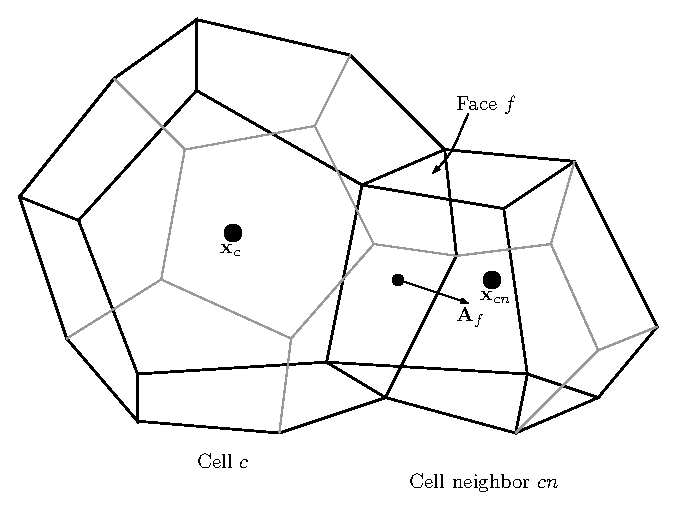
\includegraphics[width=0.5\linewidth]{figures/FaceOrientation}
\caption{Schematic of a multidimensional cell.}
\label{fig:faceorientation}
\end{figure}

\noindent
Integrating Eq. \eqref{eq:euler_operator_form} over a finite volume,
\beqn 
\int_V \biggr( 
\partialderiv{\mathbf{U}}{t} + 
\bnabla \dotp \mathcal{F}(\mathbf{U})
\biggr) dV &= 
\int_V \mathbf{Q} dV \\
\eeqn 
where $\mathcal{F} (\mathbf{U}) = \big[
\mathbf{F}(\mathbf{U}),
\mathbf{G}(\mathbf{U}), 
\mathbf{H}(\mathbf{U})
\big]$. Next, using Gauss's divergence theorem, allows us to write
\beqn
\int_V \partialderiv{\mathbf{U}}{t}  dV 
+ 
\int_S \mathbf{n} \dotp \mathcal{F}  dA &= 
\int_V \mathbf{Q} dV .
\eeqn 
Now, using cell $c$ as the volume of integration, and assuming $\mathbf{U}$ and $\mathbf{Q}$ constant over the cell, with values $\mathbf{U}_c$ and $\mathbf{Q}_c$, the above equation becomes
\beqn \label{eq:general_finite_volume}
V_c \partialderiv{\mathbf{U}_c}{t} 
+ 
\sum_{f=0}^{N_{f,c}{-}1} 
\mathbf{A}_f \dotp \mathcal{F}_f
= 
V_c \mathbf{Q}_c.
\eeqn 
where $V_c$ is the volume of the cell, $N_{f,c}$ is the number of faces for cell $c$, $\mathbf{A}_f$ is the area-vector of face $f$, which is the product of the face area, $A_f$, and the face normal, $\mathbf{n}_f$, and $\mathcal{F}_f = \mathcal{F}(\mathbf{U}_f)$ is the face flux vector.  The treatment of the $\mathcal{F}_f$ term is the topic of the MUSCL-Hancock method which we detail in section \ref{section:MHM}.

\vspace{1cm}
\subsection{Multidimensional transformation of interface fluxes}
Most of the Riemann solver schemes presented in \cite{Toro} are for one dimensional geometries. A transformation technique is prescribed in \cite{Toro} that allows one to seamlessly use the one dimensional formulations, and is as follows. 

Given the arbitrary face area vector, $\mathbf{A}_f=\mathbf{n}_f A_f$, we first seek a rotation matrix, $R_{\ihat}$, to rotate any vector about an axis $\mathbf{a}_{\ihat}$ such that it is aligned with $\ihat$. To determine $R_{\ihat}$ we first set the rotation axis as
\beqn 
\mathbf{a}_{\ihat} = \frac{\mathbf{n}_f \times \ihat}{||\mathbf{n}_f \times \ihat||}
\eeqn 
and the angle of rotation, $\theta_{\ihat}$, as
\beqn 
\theta_{\ihat} = \arccos (\mathbf{n}_f \dotp \ihat).
\eeqn 
We then apply Rodrigues's formula as detailed in appendix \ref{appendix:Roderigues_formula} to obtain $R_{\ihat}$. With this matrix in hand we can form the general transformation matrix, $T_{\ihat}$, defined as
\beqn
T_{\ihat} = \text{diag}(1,R,1) = 
\begin{bmatrix}
1 & 0         & 0         & 0         & 0 \\
0 & R_{00} & R_{01} & R_{02} & 0 \\
0 & R_{10} & R_{11} & R_{12} & 0 \\
0 & R_{20} & R_{21} & R_{22} & 0 \\
0 & 0         & 0         & 0         & 1 \\
\end{bmatrix}
\eeqn
which can be used to define 
\beqn 
\hatbf{F}_f = \mathbf{F}(\hatbf{U}_f)
\eeqn 
where
\beqn 
\hatbf{U}_f = T_{\ihat} \mathbf{U}_f
\eeqn 
such that
\beqn 
\mathbf{n}_f \dotp \mathcal{F}_f
= \mathbf{n} \dotp [
\mathbf{F}(\mathbf{U}_f),
\mathbf{G}(\mathbf{U}_f),
\mathbf{H}(\mathbf{U}_f)]
=
T_{\ihat}^{-1} \hatbf{F}_f
\eeqn 
allowing us to write Eq. \eqref{eq:general_finite_volume} as 
\beqn 
\partialderiv{\mathbf{U}_c}{t} 
+ 
\frac{1}{V_c}
\sum_{f=0}^{N_{f,c}{-}1} 
A_f  T_{\ihat}^{-1} \hatbf{F}_f
=  \mathbf{Q}_c.
\eeqn 
In this form any Riemann solver can simply be supplied with $\hat{\mathbf{U}}$ for the cells on either side of an interface in order to use the classical one dimensional formulations contained in \cite{Toro}. The given Riemann solver will then produce the appropriate value for $\hatbf{F}_f$.



%\vspace{1cm}
%\subsection{One dimensional Finite Volume discretization}
%In one dimension we will be using the indexing scheme as shown in Figure \ref{fig:mesh1d} below. Cell indices are $i\in[0, N_c-1]$ where $N_c$ is the number of cells in the problem. The indices also indicate a cell's position from left to right, $i{=}0$ denoting the left-most cell and $i{=}N_c{-1}$ denoting the right-most cell. Throughout this research we will also use \textit{virtual nodes} to indicate the interfaces between cells, these will be denoted with half indices, i.e., $i{=}\frac{1}{2}$ denotes the interface between cell $i=0$ and cell $i=1$.
%\begin{figure}[H]
%\centering
%\includegraphics[width=1.0\linewidth]{figures/Mesh1D}
%\caption{One dimensional mesh description.}
%\label{fig:mesh1d}
%\end{figure}
%Using this indexing scheme allows us to write Eq. \eqref{eq:general_finite_volume} as
%\beqn 
%\partialderiv{\mathbf{U}_i}{t} + \frac{\ihat}{\Delta x_i}  \dotp
%\biggr(
%\mathbf{F}_{i{+}\frac{1}{2}} - \mathbf{F}_{i{-}\frac{1}{2}}
%\biggr)
%= \mathbf{Q}_i
%\eeqn 
%where $\mathbf{F}_{i{+}\frac{1}{2}}$ and $\mathbf{F}_{i{-}\frac{1}{2}}$ are now the interface flux terms and are not yet defined. The definition of these interface fluxes is the topic of next section.


\newpage
\section{MUSCL-Hancock Method (MHM) and the HLLC Riemann-solver} \label{section:MHM}
The MUSCL-Hancock method is conceptually simple. It prescribes how the interface fluxes are to be computed at the beginning of a time step and then how to supply the necessary inputs to a Riemann-solver for the computation of the preserved variables at the end of the timestep.
\subsection{The MUSCL-Hancock Method}
MUSCL stands for Monotone Upstream-centered Scheme for Conservation Laws. The scheme as modified by S. Hancock gives the method its name. We will refer to this method by simply using the abbreviation $MHM$.
\newline
\newline
\noindent
The MHM has three basic steps.

\subsubsection{Step 1 - Extrapolate $\mathbf{U}$ using an estimate of the gradient ($\bnabla \mathbf{U}$) and compute the interface fluxes at time step $n$}
In general notation the extrapolation of the conserved variable for cell $c$, $\mathbf{U}_c$, to a cell face $f$, $\mathbf{U}_{f,c}$, can be computed from
\beqn 
\mathbf{U}_{f,c}^n \approx \mathbf{U}_c^n + (\position_{f} - \position_c) \dotp \big\{ \bnabla \mathbf{U} \big\}_c^n,
\eeqn 
where $\mathbf{U}_f$ is the extrapolated value of $\mathbf{U}$ at the face center, $\mathbf{U}_c$ is the finite volume cell-constant value of $\mathbf{U}$ for cell $c$, $\position_f$ is the face centroid, $\position_c$ is the cell centroid, and $\big\{ \bnabla \mathbf{U} \big\}_c$ is the gradient of $\mathbf{U}$ at the center of cell $c$.

Provided that an orthogonal mush is used, the gradient can be estimated in each cell $c$ from
\beqn 
\big\{ \bnabla \mathbf{U} \big\}_c 
\approx
\frac{1}{V_c}
\sum_{f=0}^{N_{f,c}{-1}}  
\biggr\{
\mathbf{A}_f \otimes
\biggr(
\frac{||\position_f - \position_c||}{||\position_{cn} - \position_c||} \mathbf{U}_c 
+
\frac{||\position_c - \position_f||}{||\position_{cn} - \position_c||} \mathbf{U}_{cn} 
\biggr)
\biggr\},
\eeqn 
where $V_c$ is the volume of cell $c$, $N_{f,c}$ is the number of faces for cell $c$, $A_f$ the face area-vector of face $f$ (i.e., $\mathbf{A}_f = A_f \mathbf{n}_f$), $\position_{cn}$ is the centroid of the neighboring cell $cn$ at face $f$, and finally $\mathbf{U}_{cn}$ is the finite volume cell-constant value of $\mathbf{U}$ for cell $cn$.
\newline
\newline
{\color{red} Check slope limiters. }

%To reduce spurious oscillations the estimated gradient can be limited. One such limiter is a $minmod$ limiter and can be defined as
%
%\beqn 
%\big\{ \bnabla \mathbf{U} \big\}_{min} = min
%\biggr(
%\frac{\position_{cn} - \position_c}{||\position_{cn} - \position_c||} \otimes \biggr[ \mathbf{U}_{cn} - \mathbf{U}_c \biggr] \ : \ \forall cn
%\biggr)
%\eeqn 

\subsubsection{Step 2 - Advance the conserved variables by half a time step}
Using the extrapolated values $\mathbf{U}_{f,c}^n$, compute associated transformed interface fluxes, $\hatbf{F}_f^n = \mathbf{F}(T_{\ihat} \mathbf{U}_{f,c}^n)$, after which
\beqn 
\mathbf{U}_c^{n{+}\frac{1}{2}} = \mathbf{U}_c^n - \frac{\frac{1}{2}\Delta t^n}{V_c} \sum_{f=0}^{N_{f,c}{-1}} 
\biggr(
A_f T_{\ihat}^{-1} \hatbf{F}_f^n
\biggr)
+ \frac{1}{2}\Delta t^n \mathbf{Q}.
\eeqn 
These half-time step values are then passed to a suitable Riemann solver.

\subsubsection{Step 3 - Execute a Riemann solver}
The Riemann solver computes the interface fluxes, $\hatbf{F}_f^{\mathcal{R},n{+}\frac{1}{2}}$, using $\mathbf{U}_c^{n{+}\frac{1}{2}}$, where $\mathcal{R}$ denotes the specific Riemann solver. The discontinuity across a face is treated as a one dimensional problem with a left and right side having different values for $\mathbf{U}$, i.e., $\mathbf{U}_L = \hatbf{U}_c^{n{+}\frac{1}{2}}$ and $\hatbf{U}_R = \mathbf{U}_{cn}^{n{+}\frac{1}{2}}$ for the left and right side respectively.


When using the HLLC solver, as described in \cite{Toro}, the Riemann solver will compute $\hatbf{F}_f^{hllc,n{+}\frac{1}{2}}$ after which we compute the conserved variables at $n+1$ from
\beqn 
\mathbf{U}_c^{n+1} = \mathbf{U}_c^n - \frac{\Delta t^n}{V_c} \sum_{f=0}^{N_{f,c}{-1}} 
\biggr(
A_f T_{\ihat}^{-1}
\hatbf{F}_f^{hllc,n{+}\frac{1}{2}}
\biggr)
+ \Delta t^n \mathbf{Q}.
\eeqn 
The HLLC Riemann solver is detailed in section \ref{section:HLLC}.

\newpage 
\subsection{The HLLC Approximate Riemann Solver in one dimension} \label{section:HLLC}
The Harten Lax and van Leer (HLL) solver scheme was developed in 1983 \cite{Toro} and requires estimates for the fastest wave/signal/shock velocities emerging from a discontinuity. Later Toro, Spruce and Speares proposed the Harten Lax van Leer \textit{Contact} (HLLC) scheme \cite{Toro} which adds another wave to the problem.
\newline
\newline
The primary inputs for this solver are
\beqn 
\mathbf{U}_L &= \hatbf{U}_c^{n{+}\frac{1}{2}} \\
\mathbf{U}_R &= \hatbf{U}_{cn}^{n{+}\frac{1}{2}} \\
\mathbf{F}_L &= \mathbf{F}(\hatbf{U}_{c}^{n{+}\frac{1}{2}}) \\
\mathbf{F}_R &= \mathbf{F}(\hatbf{U}_{cn}^{n{+}\frac{1}{2}}) \\
\eeqn 


\subsubsection{Fastest wave speed estimation}
The HLLC Riemann solver is predicated on knowing an estimate for the maximum wave speed, $S_{max}$, which can be computed from 
\beqn
S_{max} =\max (|{u}_L| + a_L, |{u}_R| + a_R),
\eeqn
where $a_L$ and $a_R$ are the sound speeds associated with the left- and right conserved variables as
\beqn 
a = \sqrt{\frac{\gamma p}{\rho}}.
\eeqn 

Once a value for $S_{max}$ has been determined, we can set 
\beqn 
S_L = -S_{max}
\eeqn 
and
\beqn 
S_R = S_{max}.
\eeqn 

\subsubsection{Contact wave speed}
The contact wave speed, $S_*$, is given by
\beqn 
S_* = \frac{p_R - p_L +\rho_L u_L(S_L-u_L) - \rho_R u_R(S_R-u_R)}
{\rho_L (S_L-u_L) - \rho_R(S_R-u_R)}.
\eeqn 

\subsubsection{Intermediate fluxes}
As per \cite{Toro} the intermediate fluxes, $\mathbf{F}_{*L}$ and $\mathbf{F}_{*R}$ are given by
\beqn 
F_{*K} = 
\frac
{S_* (S_K \mathbf{U}_K - \mathbf{F}_K) + S_K(p_K+\rho_L(S_K-u_K)(S_*-u_K))D_*}
{S_K - S_*}
\eeqn 
for $K=L$ and $K=R$. The vector $\mathbf{D}_*$ is a vector such that
\beqn 
\mathbf{F}(\mathbf{U}) = u \mathbf{U} + p\mathbf{D},
\eeqn 
therefore 
\beqn 
\mathbf{D}_* = [0,1,0,0,S_*]^T
\eeqn 

\subsection{Interface flux}
The interface flux $\hatbf{F}_f^{hllc}$ is now given by
\beqn 
\hatbf{F}_f^{hllc} = 
\begin{cases}
\mathbf{F}_L &,\text{ if } S_L \ge 0, \\
\mathbf{F}_{*L} &,\text{ if } S_L \le 0 \le S_*, \\
\mathbf{F}_{*R} &,\text{ if } S_* \le 0 \le S_R, \\
\mathbf{F}_R &,\text{ if } S_R \le 0
\end{cases}
\eeqn 

\newpage
\begin{thebibliography}{1}
	
%	\bibitem{LewisMiller} Lewis E.E., Miller W.F., {\em Computational Methods of Neutron Transport}, JohnWiley \& Sons, 1984
	
	\bibitem{Toro} Toro E.F., {\em Riemann Solvers and Numerical Methods for Fluid Dynamics - A Practical Introduction}, third edition, Springer, 2009.
	   
\end{thebibliography}

\newpage
\begin{appendices}
\section{Roderigues's formula} \label{appendix:Roderigues_formula}
Roderigues' formula for the rotation of a vector $\mathbf{v}$ about a unit vector $\mathbf{a}$ with right-hand rule
\begin{equation}
\newcommand{\vvec}{\mathbf{v}}
\newcommand{\avec}{\mathbf{a}}
\begin{aligned}
\vvec_{rotated} &= \cos \theta \vvec + (\avec \dotp \vvec)(1-\cos \theta) \avec + \sin \theta (\avec \times \vvec)
\end{aligned}
\end{equation}
In matrix form
\beqn 
\mathbf{v}_{rotated} = A \mathbf{v}
\eeqn 
where
\beqn 
A = 
\begin{bmatrix}
0 & -a_z & a_y \\
a_z & 0 & -a_x \\
-a_y & a_x & 0
\end{bmatrix}
\eeqn 
and
\beqn 
R = I + \sin\theta A + (1-\cos\theta) A^2
\eeqn

\end{appendices}

\end{document}